\chapter{Gestión del Proyecto}\label{cap:03gestión}

%\section{Introducción}
En este capítulo se presenta toda la información relacionada con la gestión del proyecto de la elaboración del TFG. El capítulo se divide en cuatro secciones: \ref{sec:03Participantes} Participantes del Proyecto,
%\ref{sec:03EDT} Estructura de Desglose de Trabajo, 
%\ref{sec:03Recursos} Estimación de recursos, 
\ref{sec:03Temporal} Planificación temporal, \ref{sec:03Costes} Evaluación de costes y \ref{sec:03Riesgos} Identificación de riesgos y planes de contingencia.

\section{Participantes del Proyecto} \label{sec:03Participantes}

Los participantes del proyecto TFG se presentan a continuación mediante una tabla que recoge su nombre, institución a la que pertenece, rol asignado durante la elaboración del proyecto e información de contacto. 

Es importante destacar que los tres primeros participantes corresponden a alumna y tutores de la Escuela Técnica Superior de Ingeniería Informática de la Universidad de Sevilla y los dos últimos participantes, a los tutores de las prácticas realizadas en el Departamento de Innovación Tecnológica del Hospital Universitario Virgen del Rocío.

%\begin{table}[H]
    \centering
    \begin{tabular}{|c|c|}
    \hline
    \textbf{Participante} & María del Valle Alonso de Caso Ortiz \\
    \hline
    \textbf{Institución} & Universidad de Sevilla \\
    \hline
    \textbf{Rol} & Jefe de Proyecto \& Developer \& Analista \\
    \hline
    \textbf{Información de contacto} & vallealonsodecaso@icloud.com \\ 
    \hline
    \end{tabular}
\caption{Descripción del primer participante del proyecto}
\label{tab:primerParticipante}
\end{table}

\begin{figure}[H]
    \centering
    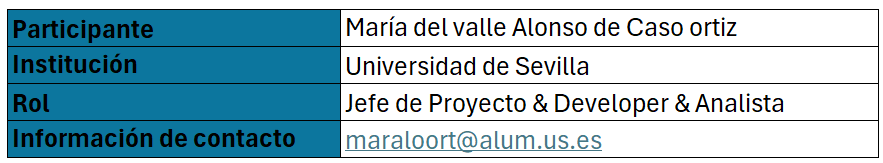
\includegraphics[width=0.80\textwidth]{tables/primerParticipante.png}
    \captionof{table}{Descripción del primer participante del proyecto}
    \label{table:primerParticipante}
\end{figure}

\begin{figure}[H]
    \centering
    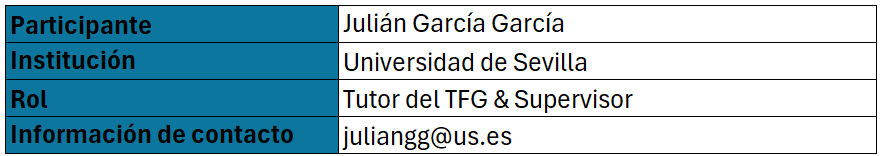
\includegraphics[width=0.80\textwidth]{tables/segundoParticipante.png}
    \captionof{table}{Descripción del segundo participante del proyecto}
    \label{table:segundoParticipante}
\end{figure}

\begin{figure}[H]
    \centering
    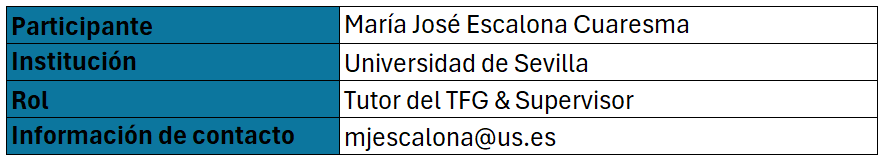
\includegraphics[width=0.80\textwidth]{tables/tercerParticipante.png}
    \captionof{table}{Descripción del tercer participante del proyecto}
    \label{table:tercerParticipante}
\end{figure}

\begin{figure}[H]
    \centering
    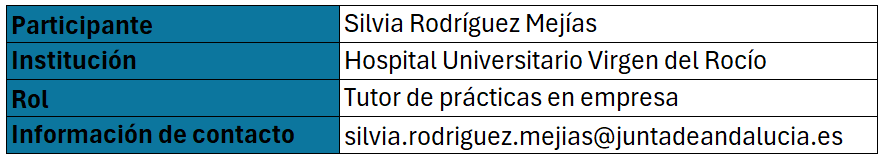
\includegraphics[width=0.80\textwidth]{tables/cuartoParticipante.png}
    \captionof{table}{Descripción del cuarto participante del proyecto}
    \label{table:cuartoParticipante}
\end{figure}

\begin{figure}[H]
    \centering
    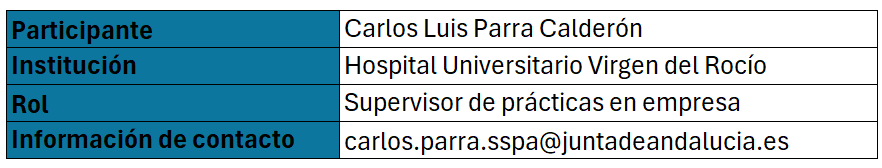
\includegraphics[width=0.80\textwidth]{tables/quintoParticipante.png}
    \captionof{table}{Descripción del quinto participante del proyecto}
    \label{table:quintoParticipante}
\end{figure}
%\section{Estructura de desglose de trabajo} \label{sec:03EDT}

\section{Planificación temporal} \label{sec:03Temporal}

La planificación temporal se realiza dentro del marco de la asignatura Trabajo de Fin de Grado que consta de 12 créditos ECTS y una duración aproximada de 300 horas. Además, el trabajo se ha realizado de forma linear y combinada con las prácticas curriculares, de 13.5 créditos ECTS y 337 horas, por lo que la planificación contempla ambas tareas de forma conjunta.

Para ello se realiza una planificación basada en cuatro sprints, de cuatro semanas de duración cada uno. De esta forma se pretende tener cada mes un nuevo incremento del proyecto y con ello, un feedback por parte del product owner (véase \ref{cap:04metodologia}). 

El comienzo del proyecto se estima al fin de las vacaciones de navidad, el 10 de enero de 2024. De esta forma, se estima que la duración del proyecto será de 4 meses, con intención de ser entregado en la primera convocatoria de Trabajo Fin de Grado en mayo de 2024.

Es importante comentar que aunque todos los sprint guardan la misma duración (cuatro semanas), no todos los sprint estiman un esfuerzo igual, puesto que el producto y sus requisitos van incrementando en cada sprint, de modo que en los primeros sprint se estima una carga de trabajo menor (más ligada a la investigación) mientras que en los últimos sprint, más próximos a la fecha de entrega y con un incremento de producto mayor, se estima mayor esfuerzo.

A continuación se presenta una tabla descriptiva para cada sprint, con la planificación temporal y la dedicación real. 

\begin{figure}[H]
    \centering
    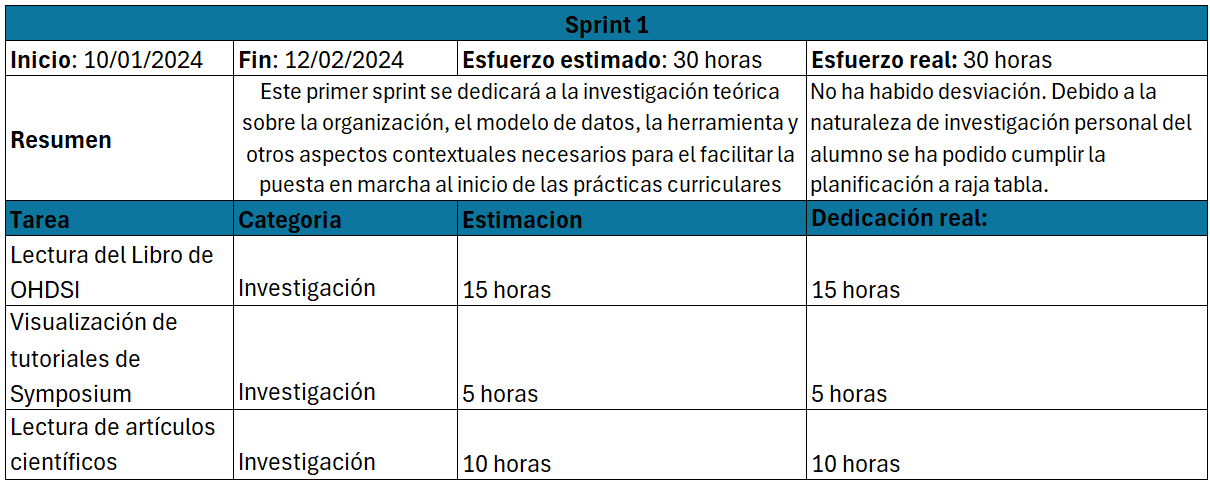
\includegraphics[width=1\textwidth]{tables/sprint1cap.png}
    \captionof{table}{Planificación y dedicación real del primer sprint}
    \label{table:sprint1cap}
\end{figure}

\begin{figure}[H]
    \centering
    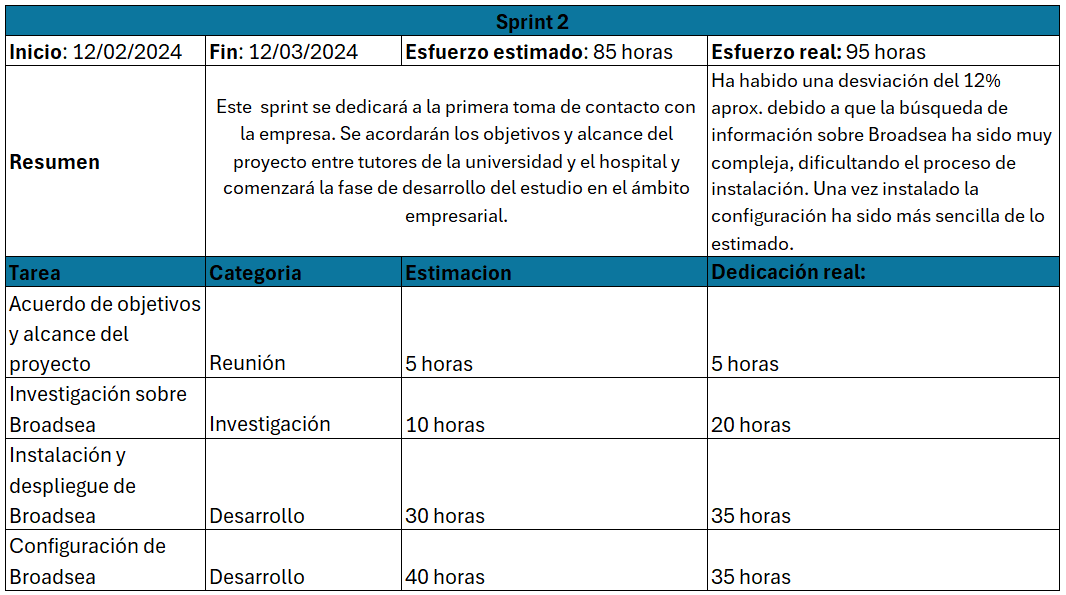
\includegraphics[width=1\textwidth]{tables/sprint2cap.png}
    \captionof{table}{Planificación y dedicación real del segundo sprint}
    \label{table:sprint2cap}
\end{figure}

\begin{figure}[H]
    \centering
    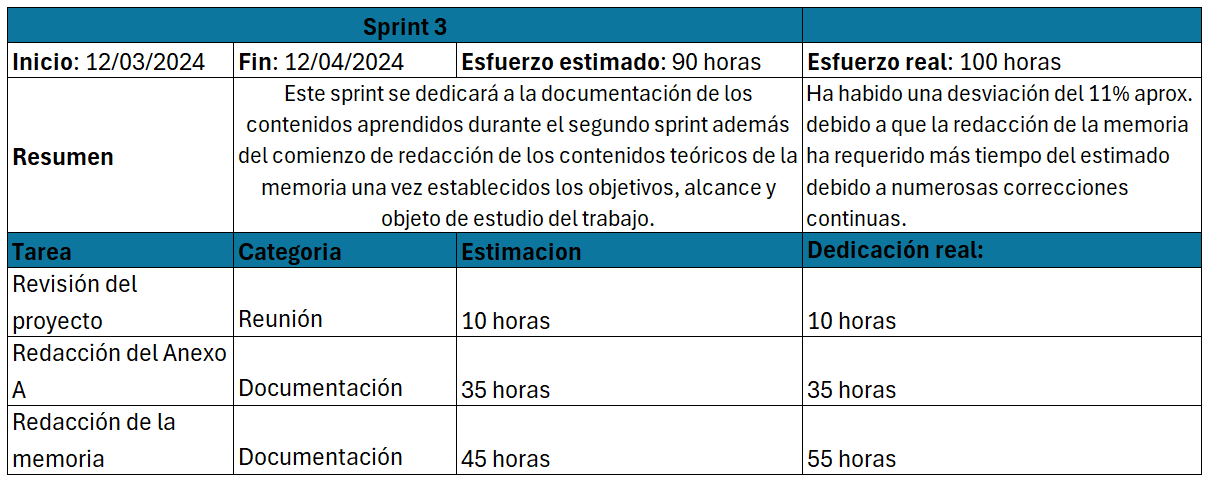
\includegraphics[width=1\textwidth]{tables/sprint3cap.png}
    \captionof{table}{Planificación y dedicación real del tercer sprint}
    \label{table:sprint3cap}
\end{figure}

\begin{figure}[H]
    \centering
    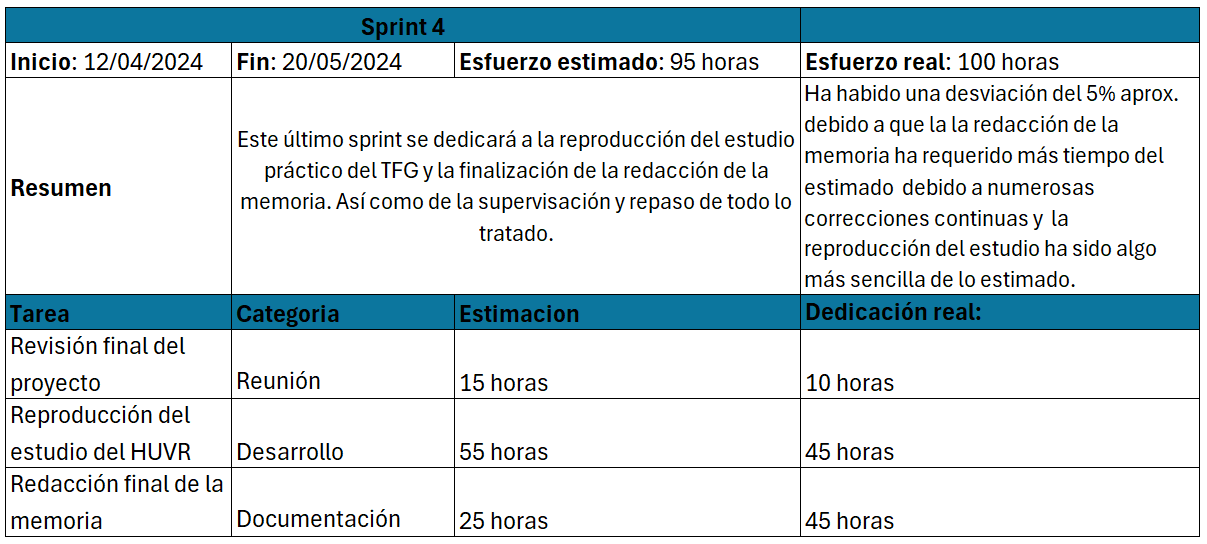
\includegraphics[width=1\textwidth]{tables/sprint4cap.png}
    \captionof{table}{Planificación y dedicación real del cuarto sprint}
    \label{table:sprint4cap}
\end{figure}

Las horas totales de trabajo planificado fueron 300 horas, según los créditos asignados a la asignatura. No obstante, la dedicación real al proyecto ha sido superior a lo previsto, dedicándole \textbf{325 horas reales}, es decir, 25 horas extra suponiendo una \textbf{desviación aproximadamente del 8\% sobre lo planificado}. Esta desviación no se considera un impedimento o anormalidad dentro de los riesgos previstos del proyecto, lo que no ha supuesto ningún impedimento mayor para la finalización del trabajo.

\section{Planificación financiera} \label{sec:03Costes}

La planificación financiera se realiza de forma similar a la elaboración de un presupuesto sobre el proyecto. Para ello se realizará el cálculo de dos tipos de coste: personal y material. Por último se esitmará el coste total y el beneficio.

\subsubsection{Coste de personal}

Para el coste de personal se tendrán en cuenta los roles definidos previamente (véase \ref{sec:03Participantes}). Concretamente, intervendrán los roles ejercidos por la alumna y se omitirán los roles de tutorización y supervisaje para el cómputo del presupuesto del proyecto.

Por tanto, el proyecto requiere del ejercicio fundamental de tres roles: jefe de proyecto, developer y analista. El jefe de proyecto asume las tareas de comunicarse con los tutores (de la universidad y del hospital), tomar decisiones y acordar objetivos y elaboración de la investigación y desarrollo téorico de la memoria del proyecto. El developer asume las tareas de instalar, desplegar y configurar el sistema así como gestionar y administrar las bases de datos, asegurar el correcto funcionamiento de la herramienta y reflejarlo en la memoria. Por último, el analista realiza las tareas meramente análiticas, se encarga de la reproducción del estudio clínico y su redacción en la memoria \textit{per se} haciendo uso de la herramienta una vez instalada.

Los costes de cada rol se calculan por hora, utilizando como referencia el precio medio publicado en la consulta preliminar para perfiles profesionales del ámbito informático \cite{informeJuntaAndalucia}, considerando la categoría junior para cada uno. 

A continuación se presenta en negrita el rol definido en el proyecto seguido de la categoría a la que se ha asociado según el informe de la Junta y el coste total asociado a las horas reales invertidas en sus tareas, según lo estipulado en la planificación temporal (véase \ref{sec:03Temporal}).

\begin{itemize}
    \item \textbf{Jefe de proyecto.} Jefe de proyecto y coordinador junior: 39.16€/h.

%\begin{equation}
%   39.16 \, \text{€/h} \times 110 \, \text{h} = 4307.60 \, \text{€}
%\end{equation}

    \item \textbf{Developer.} Administrador de la base de datos junior: 35.18€/h.

%\begin{equation}
%    35.18 \, \text{€/h} \times 125 \, \text{h} = 4397.50 \, \text{€}
%\end{equation}

    \item \textbf{Analista.} Analista funcional de aplicaciones junior: 33.12€/h

%\begin{equation}
%    33.12 \, \text{€/h} \times 90 \, \text{h} = 2980.80 \, \text{€}
%\end{equation}

\end{itemize}

\begin{figure}[H]
    \centering
    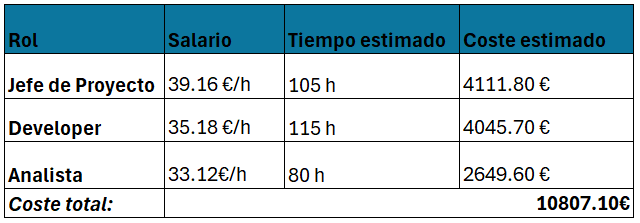
\includegraphics[width=0.90\textwidth]{tables/costeEstimcap.png}
    \captionof{table}{Coste estimado de personal del proyecto}
    \label{table:costeEstimcap}
\end{figure}

Por tanto, el \textbf{coste estimado de personal del proyecto es 10807.10€}.

%\begin{table}[H]
    \resizebox{columnwidth}{!}{%
    \centering
    \begin{tabular}{|c|c|c|c|}
    \hline
    \textbf{Rol del proyecto} & \textbf{Horas estimadas} & \textbf{Coste por hora} & \textbf{Coste total} \\
    \hline
    Jefe de proyecto & h & 39.16€/h & € \\
    \hline
    Developer & h & 35.18€/h & € \\
    \hline
    Analista & h & 33.12€/h & €\\
    \hline
    \end{tabular}
    %\begin{tabular}{|c|c|}
    %\hline
    %\textbf{Coste total} & €\\
    %\hline
    %\end{tabular}
\caption{Planificación del coste de personal total}
\label{tab:objetivosTFG}
\end{table}


\subsubsection{Coste material}

En cuanto a los costes materiales, se distinguen otras tres categorías: costes de amortizaciones, de licencias y de servicios. Es importante recordar que la planificación temporal marca una duración estimada del proyecto de cuatro meses.

En primer lugar, el coste de amortizaciones tendrá en cuenta únicamente el equipo portátil utilizado para el desarrollo del proyecto. Se realizará una amortización lineal en 5 años, con un coste inicial de 1000 € y un valor residual del 20 de este coste inicial que da lugar a un coste de 13.33€/mes.

\begin{itemize}
    \item \textbf{Equipo portátil.} Ordenador con procesador 7th generation y 8 gb de RAM.
\end{itemize}

\begin{equation}
    \text{valor residual} = 1000 \text{€} \times 0.20 = 200 \text{€}
\end{equation}

\begin{equation}
    \text{valor amortización} = \frac{1000 \text{€} - 200 \text{€}}{60 \text{ meses}} = 13.33 \text{€/mes}
\end{equation}

Por tanto, con una duración de cuatro meses, \textbf{el coste total de amortizaciones es 53.32€}

En segundo lugar, el coste de licencias tendrá en cuenta el uso de software de pago. La mayoría de las herramientas utilizadas durante el proyecto poseen un plan gratuito o son gratuitas en sí mismas, a excepción de las siguientes:

\begin{itemize}
    \item \textbf{Licencia de Windows 11 Pro} \cite{licenciaWindows}: 259€
    \item \textbf{Licencia profesional de Enterprise Architect} \cite{licenciaEA}: 229€
    \item \textbf{Licencia de Latex Estándar} \cite{licenciaOffice}: 19€/mes

\begin{equation}
    19 \, \text{€/mes} \times 4 \, \text{meses} = 76 \, \text{€}.
\end{equation}
    
\end{itemize}

Por tanto, el \textbf{coste total de licencias es 564€}.

En tercer lugar, los costes de servicios incluyen los gastos por suministro eléctrico, el cual tiene un coste promedio de 0,182 € / KWh (OCU, 2022) . Se estima un consumo medio de 0,3 KWh de los dispositivos electrónicos usados durante el desarrollo.

\begin{itemize}
    \item \textbf{Suministro eléctrico.}
\end{itemize}

\begin{equation}
0.182 \, \text{€/kWh} \times 0.3 \, \text{kWh} \times 300 \, \text{h} = 16.38 \, \text{€}.
\end{equation}

También es necesario tener en cuenta el servicio de internet, para el que se tiene contratado un servicio de fibra óptica simétrica de 100 megabytes con un coste mensual de 25,70 €:

\begin{itemize}
    \item \textbf{Suministro de internet.}
\end{itemize}

\begin{equation}
25.70 \, \text{€/mes} \times 4 \, \text{meses} = 102.8 \, \text{€}.
\end{equation}

Por tanto, el \textbf{coste total de servicios es 119.18€}

En total se obtiene un \textbf{coste material estimado de 736,50€}.

\subsubsection{Coste total y beneficio}

Sumando los costes de personal y materiales, se tiene que el \textbf{coste total estimado del proyecto asciende a la cifra de 11543.60 €}.

\begin{equation}
    10807.10\text{€} + 729.50\text{€} =  11536.60 \text{€}
\end{equation}

En cuanto al beneficio que se estima obteenr de este proyecto, se computa como el coste total más un 15\% de beneficio íntegro para la empresa. Esto hace un total de 13274,09 € de beneficio total del proyecto.

Por último, se añadirá un fondo de contingencia frente a riesgos del proyecto que quedará excluido de este coste total. Su finalidad será evitar que alguna desviación o problema pueda provocar una finalización temprana del proyecto. Corresponderá al 10\% del coste total estimado, por lo que se contará con un fondo de contingencia de 1154,36 €.

\subsubsection{Desviaciones}

El proyecto ha sufrido una desviación del 8\% sobre el tiempo en horas planificado para su conclusión (véase \ref{sec:03Temporal}. Esta desviación influye en los costes materiales, necesitándose recalcular algunos costes estimados, como el coste de personal y el de suministro eléctrico. 

En cuanto al coste de personal, el coste real ascendería a 11685.90€.% es decir una desviación del 8\% sobre el coste estimado.

\begin{figure}[H]
    \centering
    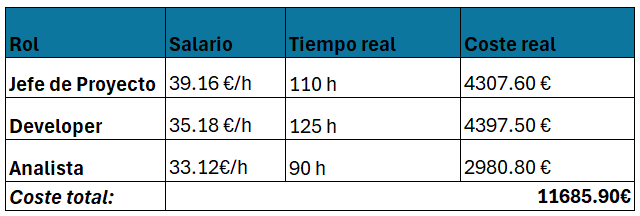
\includegraphics[width=0.90\textwidth]{tables/costeRealcap.png}
    \captionof{table}{Coste real de personal del proyecto}
    \label{table:costeRealcap}
\end{figure}

En cuanto al coste de suministro de eléctrico, el coste ascendería de forma insignificante a 17,75 €, contribuyendo a coste material de 737.87 €. 

\begin{equation}
0.182 \, \text{€/kWh} \times 0.3 \, \text{kWh} \times 325 \, \text{h} = 17,75 \, \text{€}.
\end{equation}

Por tanto, sumando las desviaciones en costes de personal y material, \textbf{el coste total real del proyecto resultaría en 12423.77 €}.

\begin{equation}
    11685.90 \text{€} + 737.87\text{€} =  12423.77 \text{€}
\end{equation}

El coste final del proyecto supone una\textbf{ desviación de 880.17 €} sobre el coste estimado del proyecto, que correspondía a 11543.60 €. No obstante, esta desviación no ha supuesto ningún riesgo para el proyecto debido a que el valor económico de la desviación no supera el valor reservado en el fondo de contingencia (1154,36). Por tanto se puede concluir que el proyecto se ha concluido de forma exitosa.

\section{Identificación de riesgos y planes de contingencia} \label{sec:03Riesgos}

Por último, para la gestión exitosa de un proyecto es importante identificar los posibles riesgos durante la elaboración del proyecto y premeditar planes de contigencia para actuar contra ellos. 

A continuación se muestra en una tabla el conjunto de posibles riesgos identificados, acompañado de una descripción y un plan de contingencia frente al mismo.

\begin{figure}[H]
    \centering
    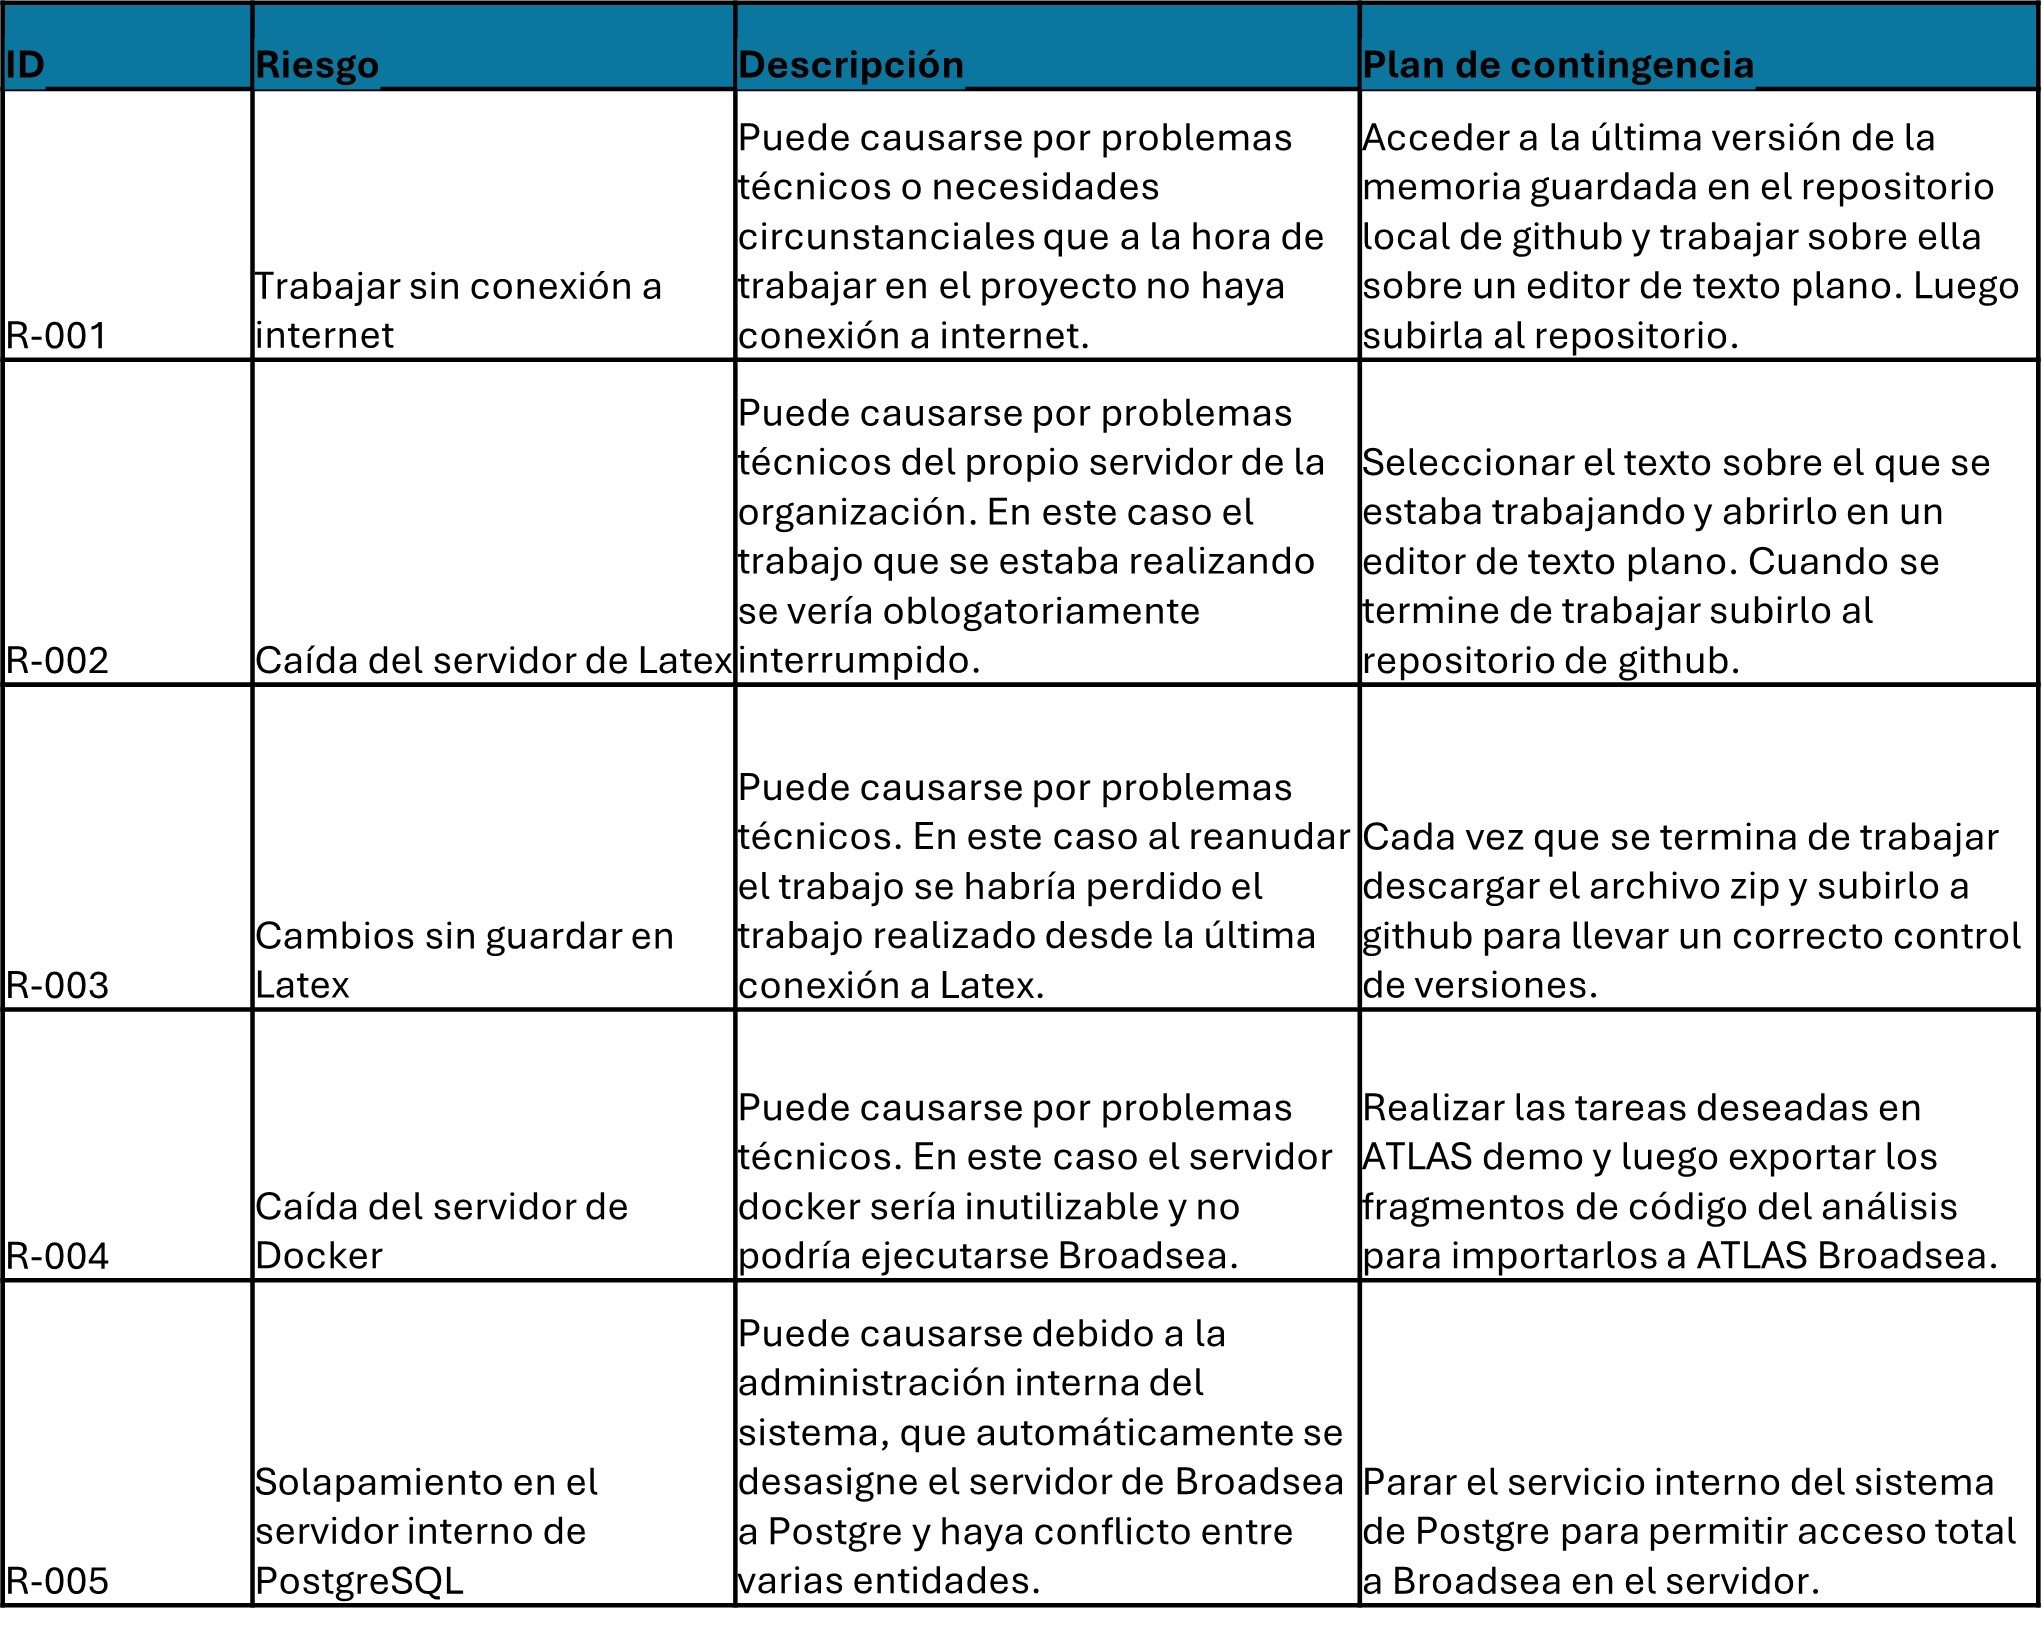
\includegraphics[width=0.90\textwidth]{tables/tablaRiesgos.jpg}
    \captionof{table}{Tabla de posibles riesgos y planes de contingencia}
    \label{table:tablaRiesgos}
\end{figure}

Una vez se han identificado los posibles riesgos se pueden ordenar y evaluar en una matriz de impacto, según el impacto que ocasionaría el riesgo y la frecuencia con la que se produce.

\begin{figure}[H]
    \centering
    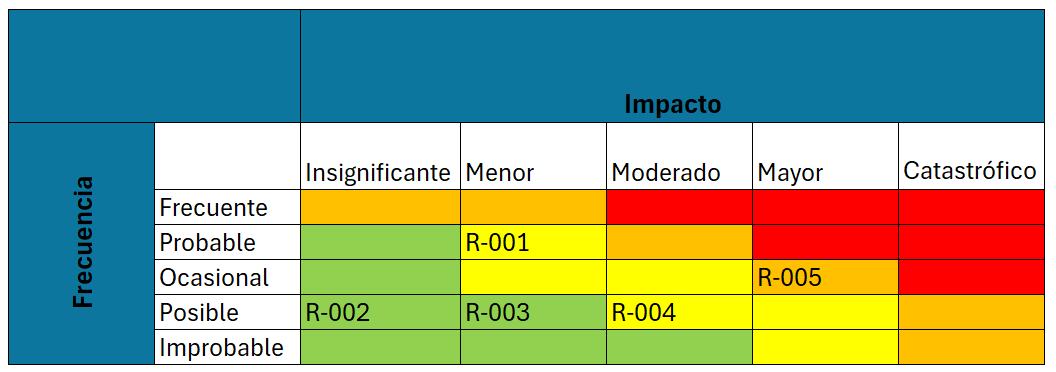
\includegraphics[width=0.80\textwidth]{tables/matrizImpacto.png}
    \captionof{table}{Matriz de impacto}
    \label{table:matrizImpacto}
\end{figure}

Puede observarse que no se ha identificado ningún riesgo catastrófico que pueda suponer un problema real para el desarrollo del proyecto, por lo que este se desarrollara potencialmente de forma segura.